% DOC OPTIONS
\documentclass[a4paper,12pt]{article} % Page Setup
\usepackage[portuguese]{babel} % Commands Language
\usepackage{graphicx} % Image Load
\usepackage[colorlinks=true,linkcolor=black,urlcolor=blue]{hyperref} % References
\usepackage[none]{hyphenat} % Remove Hyphenation
\usepackage[left=2cm,right=2cm,bottom=2cm]{geometry} % Custom margin size
\usepackage{float} % Figures and Objects better position
\usepackage{titlesec} % Figures and Objects better position
\usepackage{array} % Handle advanced table configurations
\usepackage{pdfpages} % Attach PDF's

% Table of Contents Configuration
\setcounter{tocdepth}{3} % Setting table of contents depth to 3 instead of 2

% DOCUMENT
\begin{document}

\begin{titlepage}
	\centering
	\Large \textbf{INSTITUTO POLITÉCNICO DE SETÚBAL} \\
	\normalsize \textbf{ESCOLA SUPERIOR DE TECNOLOGIAS DE SETÚBAL} \\
	\vspace{2cm}
	\begin{figure}[H]
		\centering
		
\includegraphics[scale=.5]{images/IPSLogo.png}
	\end{figure}
	\vspace{1cm}
	\Large \textbf{Qualidade de Software}\\
	\Large \textbf{Mestrado em Engenharia de Software}\\
	\vspace{1.5 cm}
	\Large Daniel Singh - 201901071\\
	\Large Rafael Marçalo - 201900456\\
	\vspace{.5cm}
	\large \today
\end{titlepage}

\newpage
\tableofcontents

\newpage
\listoffigures

\newpage
\listoftables

\newpage
\section{Introdução}
Este relatório tem como objetivo a análise da qualidade de código de um projeto realizado por outros alunos. Para esta análise iremos recorrer a ao teste de funcionalidades e requisitos do projeto. Em seguida iremos testar várias ferramentas e livrarias na análise da qualidade/consistência do código. De seguida iremos em breve apresentar não só as funcionalidades destas ferramentas, mas também os resultados que obtivemos com elas.

\newpage
\section{Análise do Caso de Estudo}
Sendo esta a primeira fase desta pequena investigação, transferi-mos o projeto caso de estudo do \textbf{Moodle}\footnote{\url{https://moodle.ips.pt/2324/}}, importámos para o nosso repositório \textbf{GitHub}\footnote{\url{https://github.com/MES-ES/QS_Lab1}} e instalámos nas nossas máquinas para análise. Desta forma, após instalarmos e configurarmos o projeto nos nossos computadores, fizemos um breve teste das suas funcionalidades e diagnosticámos alguns problemas que possam afetar a qualidade do projeto, desta forma, para simplificar o processo, elaborámos umas tabelas com o requisitos funcionais que detetamos.

\subsection{Análise de Requisitos}
\begin{table}[H]
	\centering
	\begin{tabular}{|l|p{12cm}|l|r|}
		\hline
		\textbf{ID} & \textbf{Descrição} & \textbf{Implementado}\\
		\hline
		RF1 & O sistema deverá permitir inserir novos clientes & Sim \\
		\hline
		RF2 & O sistema deverá permitir pesquisar pelos clientes & Sim \\
		\hline
		RF3 & O sistema deverá permitir aplicar filtros às pesquisas dos clientes & Parcialmente\footnotemark \\
		\hline
		RF4 & O sistema deverá permitir atualizar a informação dos clientes & Sim \\
		\hline
		RF5 & O sistema deverá permitir eliminar clientes & Sim \\
		\hline
		RF6 & O sistema deverá efetuar a validação de dados ao criar um cliente & Parcialmente\footnotemark \\
		\hline
		RF7 & O sistema deverá limpar os campos prévios dos formulários, após sua utiliazação & Não \\
		\hline
	\end{tabular}
	\caption{Análise de requisitos entidade cliente}
\end{table}

\begin{table}[H]
	\centering
	\begin{tabular}{|l|p{12cm}|l|r|}
		\hline
		\textbf{ID} & \textbf{Descrição} & \textbf{Implementado}\\
		\hline
		RF8 & O sistema deverá permitir inserir novos utilizadores & Sim \\
		\hline
		RF9 & O sistema deverá permitir pesquisar pelos utilizadores & Sim \\
		\hline
		RF10 & O sistema deverá permitir aplicar filtros às pesquisas dos utilizadores & Parcialmente\footnotemark[2] \\
		\hline
		RF11 & O sistema deverá permitir atualizar os seus dados pessoais & Não \\
		\hline
		RF12 & O sistema deverá permitir não atualizar os dados pessoais de utilizadores com as mesmas roles ou com hierarquia superior & Não \\
		\hline
		RF13 & O sistema deverá permitir atualizar a informação de outros utilizadores com hierarquia inferior & Sim \\
		\hline
		RF14 & O sistema deverá permitir eliminar outros utilizadores & Sim \\
		\hline
		RF15 & O sistema deverá efetuar a validação de dados ao criar um utilizador & Parcialmente\footnotemark[3] \\
		\hline
		RF16 & O sistema deverá limpar os campos prévios dos formulários, após sua utiliazação & Não \\
		\hline
	\end{tabular}
	\caption{Análise de requisitos entidade utilizador}
\end{table}

\footnotetext[2]{Utiliza biblioteca externa}
\footnotetext{Apenas no lado do cliente}

\begin{table}[H]
	\centering
	\begin{tabular}{|l|p{12cm}|l|r|}
		\hline
		\textbf{ID} & \textbf{Descrição} & \textbf{Implementado}\\
		\hline
		RF17 & O sistema deverá permitir criar serviços & Sim \\
		\hline
		RF18 & O sistema deverá permitir pesquisar pelos serviços & Sim \\
		\hline
		RF19 & O sistema deverá permitir realizar pesquisas filtrados aos serviços & Sim \\
		\hline
		RF20 & O sistema deverá permitir aplicar filtros às pesquisas dos serviços & Sim \\
		\hline
		RF21 & O sistema deverá permitir atualizar a informação dos serviços & Sim \\
		\hline
		RF22 & O sistema deverá de validar os dados ao criar um serviço & Sim \\
		\hline
		RF23 & O sistema deverá permitir reabrir um serviço concluído & Sim \\
		\hline
		RF24 & O sistema deverá de mostrar qual o index do serviço relativamente à sua prioridade & Parcialmente\footnotemark \\
		\hline
		RF25 & O sistema deverá limpar os campos prévios dos formulários, após sua utiliazação & Não \\
		\hline
	\end{tabular}
	\caption{Análise de requisitos entidade serviço}
\end{table}

\begin{table}[H]
	\centering
	\begin{tabular}{|l|p{12cm}|l|r|}
		\hline
		\textbf{ID} & \textbf{Descrição} & \textbf{Implementado}\\
		\hline
		RF26 & O sistema deverá permitir enviar mensagens para outros utilizadores em tempo real & Sim \\
		\hline
		RF27 & O sistema deverá permitir escolher para qual utilizador enviar mensagem & Sim \\
		\hline
		RF28 & O sistema deverá permitir visualizar o histórico de mensagens & Sim \\
		\hline
		RF29 & O sistema deverá permitir mensagens de grupo & Não \\
		\hline
	\end{tabular}
	\caption{Análise de requisitos entidade mensagem}
\end{table}

\begin{table}[H]
	\centering
	\begin{tabular}{|l|p{12cm}|l|r|}
		\hline
		\textbf{ID} & \textbf{Descrição} & \textbf{Implementado}\\
		\hline
		RF30 & O sistema deverá permitir fazer login & Parcialmente\footnotemark[4] \\
		\hline
		RF31 & O sistema deverá permitir fazer logout & Parcialmente\footnotemark[4] \\
		\hline
		RF32 & O sistema deverá de verificar permissões no routing & Não \\
		\hline
	\end{tabular}
	\caption{Análise de requisitos entidade sistema}
\end{table}
\footnotetext{Está implementado mas não funciona corretamente}

\newpage
\section{Ferramentas de Análise}
Após um diagnóstico de requisitos do projeto, avançamos para uma análise a nível de possíveis problemas de código, para esta tarefa, efetuamos uma pesquisa de ferramentas que nos possam ajudar com este trabalho, das quais, achamos importante destacar:

\begin{itemize}
	\item \textbf{ESLint} é uma ferramenta de análise de código estático que verifica o código JavaScript procurando diversos problemas comuns, como erros de sintaxe, problemas de formatação, violações de estilo de código e possíveis bugs.

	\item \textbf{Prettier Code Formatter} é um formatador de código. Impõe um estilo consistente analisando o código e reescrevendo-o conforme um conjunto de regras que levam em consideração diversos parâmetros como (comprimento máximo de linha, agrupando o código quando necessário, etc...). Ao utilizarmos esta ferramenta conseguimos garantir a uniformização do código desenvolvido ao longo do projeto.

	\item \textbf{Jest} é uma framework para testes de código compatível com bastantes projetos (Babel, TypeScript, Node, React, Angular, Vue e mais...). Suporta mocking, gera reports de code coverage.

	\item \textbf{Mocha} é outra framework de testes para Node capaz de correr no browser. Esta framework contém “interfaces” de testes que podem ser utilizados para vários tipos de desenvolvimento(TDD, BDD, exports, qunit, require, etc...). O Mocha também permite o fácil teste de funções assíncronas e de promises.

	\item \textbf{Chai}, livraria de testes especificada para testes do tipo BDD/TDD, esta livraria geralmente é integrada noutras frameworks específicas de testes(como o Mocha, por exemplo).
\end{itemize}

\newpage
\section{Linting}
Para a análise de linting do código usamos a ferramenta ESLint, devido à sua alta configurabilidade e por ser uma das ferramentas de linting mais utilizadas, como podemos observar no esquema abaixo:

\vspace{1cm}
\begin{figure}[H]
	\centering
	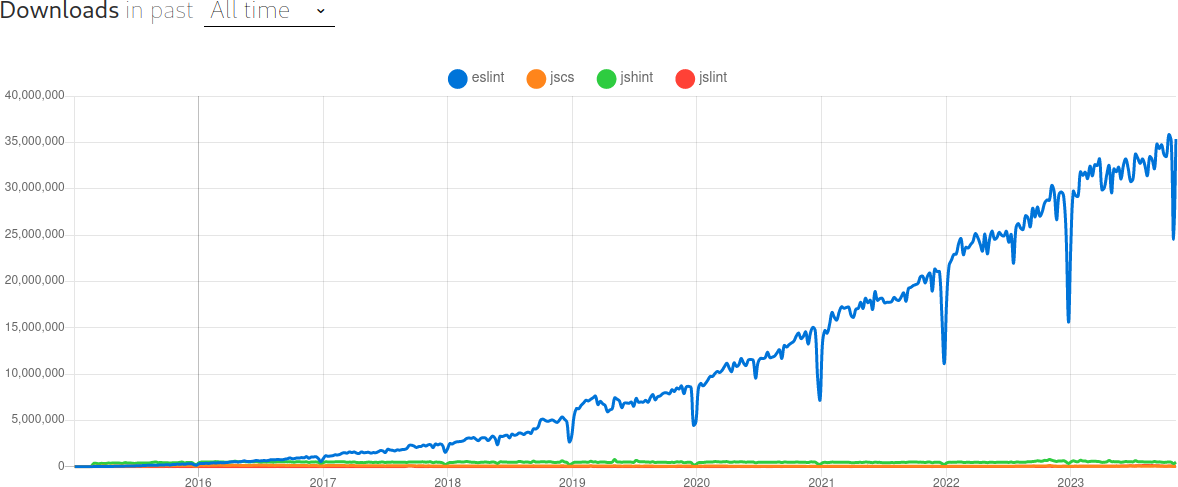
\includegraphics[scale=1.5]{images/lintTrend.png}
	\caption[Estatísticas de Download de Linters]{Estatísticas do download dos Linters ao longo do tempo\footnotemark}
\end{figure}
\vspace{1cm}
\footnotetext{Imagem obtida através de \url{https://npmtrends.com/eslint-vs-jscs-vs-jshint-vs-jslint}}

A nossa experiência a utilizar o \textbf{ESLint} tem sido bastante benéfica, ajudou-nos a identificar vários problemas no código analisado. Devido a configurabilidade da ferramenta, esta permitiu-nos identificar e relatar diversos problemas desde erros de sintaxe a problemas mais complexos relacionados com a qualidade e a manutenibilidade do código \textbf{JavaScript}. Adicionalmente podemos também referir que a habilidade de definir regras personalizadas ajudaram-nos a adaptar a ferramenta aos requisitos do projeto.

Com a ajudar deste \href{https://stackoverflow.com/a/62453095}{custom formatter} foi nos possível organizar os resultados obtidos do output do \textbf{ESLint}.

\newpage
\subsection{Resultados}
Através desta ferramenta, foi nos possível efetuar várias auditorias ao código utilizando várias configurações, permitindo-nos assim destacar as estatísticas

\subsubsection{Análise simples}
Para esta análise, configuramos o \textbf{ESLint} para apenas reportar erros de sintaxe e alguns problemas de código em geral(variáveis inutilizadas, valores \textit{undefined}, \textit{espaços} misturados com \textit{tabs}, etc...).

\vspace{1cm}
\begin{table}[H]
	\centering
	\begin{tabular}{|l|r|}
		\hline
		\textbf{Problema Anotado} & \textbf{Total} \\
		\hline
		Variáveis Inutilizadas & 40 \\
		\hline
		Valores \textit{undefined} & 189 \\
		\hline
		\textit{Espaços} Misturados com \textit{Tabs} & 2 \\
		\hline
	\end{tabular}
	\caption{Análise de Lint Simples}
\end{table}

\subsubsection{Análise simples (Client-side)}
Nesta análise decidimos fazer distinção entre problemas de código de cliente obtendo assim os seguintes resultados:

\vspace{1cm}
\begin{table}[H]
	\centering
	\begin{tabular}{|l|r|}
		\hline
		\textbf{Problema Anotado} & \textbf{Total} \\
		\hline
		Variáveis Inutilizadas & 23 \\
		\hline
		Valores \textit{undefined} & 189 \\
		\hline
		\textit{Espaços} Misturados com \textit{Tabs} & 2 \\
		\hline
	\end{tabular}
	\caption{Análise de Lint Simples (Client-side)}
\end{table}

\newpage
\subsubsection{Análise simples (Server-side)}
Nesta análise decidimos fazer distinção entre problemas de código de servidor obtendo assim os seguintes resultados:

\vspace{1cm}
\begin{table}[H]
	\centering
	\begin{tabular}{|l|r|}
		\hline
		\textbf{Problema Anotado} & \textbf{Total} \\
		\hline
		Variáveis Inutilizadas & 17 \\
		\hline
	\end{tabular}
	\caption{Análise de Lint Simples (Server-side)}
\end{table}

\subsubsection{Análise detalhada}
Para a análise detalhada, configuramos o \textbf{ESLint} para reportar os problemas da análise simples, assim como os problemas de estilo de código. Para esta análise, escolhemos os estilo de código \hyperlink{https://github.com/standard/standard}{\textit{Standard}} onde pudemos observar os seguintes resultados:

\vspace{1cm}
\begin{table}[H]
	\centering
	\begin{tabular}{|l|r|}
		\hline
		\textbf{Problema Anotado} & \textbf{Total} \\
		\hline
		Utilização de \textit{aspas} & 772 \\
		\hline
		Utilização de \textit{ponto e vírgula} & 1302 \\
		\hline
		\textit{Espaço} a terminar linha & 171 \\
		\hline
		Linhas em branco & 26 \\
		\hline
		Indentação incorreta & 2062 \\
		\hline
		\textit{Espaço} inserido várias vezes de seguida & 11 \\
		\hline
		\textit{Espaço} inserido antes de comentário & 50 \\
		\hline
		\textit{Espaço} em falta antes do \textit{parênteses} da \textit{função} & 121 \\
		\hline
		\textit{Espaço} em falta antes de blocos de código & 67 \\
		\hline
		Operador ternário desnecessário & 1 \\
		\hline
		Trocar variável para \textit{const} & 1 \\
		\hline
		Usar \textit{var} & 11 \\
		\hline
		\textit{Espaço} antes de uma palavra-chave & 2 \\
		\hline
		Estilo das \textit{chavetas} & 93 \\
		\hline
		\textit{Espaço} entre as \textit{=>} & 85 \\
		\hline
		\textit{Objeto} abreviado & 6 \\
		\hline
		Caractere terminal de ficheiro & 5 \\
		\hline
		\textit{Espaço} dentro da definição de objeto & 5 \\
		\hline
		Variáveis Inutilizadas & 11 \\
		\hline
		\textit{Espaços} \textit{padding} blocos de código & 7 \\
		\hline
		\textit{Hardcoded callback} & 24 \\
		\hline
		Valores \textit{undefined} & 189 \\
		\hline
		Propriedades sem \textit{aspas} & 6 \\
		\hline
		\textit{Tabs} vazios & 2 \\
		\hline
		Nova linha após \textit{parênteses} de objeto & 9 \\
		\hline
		Nova linha após propriedade de objeto & 9 \\
		\hline
		Falta de \textit{espaços} entre operadores lógicos e aritméticos & 22 \\
		\hline
		\textit{Vírgula} em propriedades finais de objetos & 2 \\
		\hline
		\textit{Espaços} entre parênteses & 2 \\
		\hline
		\textit{Espaços} múltiplos & 2 \\
		\hline
	\end{tabular}
	\caption{Análise de Lint Detalhada}
\end{table}

\newpage
\subsubsection{Análise dos resultados obtidos}
Observando a análise de código detalhada podemos constatar que muitos dos problemas apontados pela ferramenta, poderiam ser evitados através da utilização de uma ferramenta de formatação de código \textit{(ex: \textbf{Prettier Code Formatter})}.

\hfill

O \textbf{Prettier} é uma ferramenta de formatação de código que analisar o código e de seguida, o imprime de novo num estilo consistente. Ao contrário dos linters tradicionais que se focam em identificar e corrigir erros de codificação específicos, o principal objetivo do \textbf{Prettier} é impor um estilo de código consistente e opinativo em todo o código-fonte.

Um dos principais benefícios do \textbf{Prettier} é a sua simplicidade e configuração \textit{barebones}. Ele pretende minimizar a necessidade dos programadores tomarem decisões sobre o estilo de código, fornecendo um conjunto padrão de regras sendo estas facilmente configuradas.

Os programadores podem integrar o \textbf{Prettier} no seu \textit{workflow} usando-o diretamente a partir da linha de comandos ou integrando-o diretamente em editores de código e \textit{IDEs}.

\newpage
\section{Normas ISO}
As normas ISO em desenvolvimento de software são padrões internacionais que permitem aos programadores de todo o mundo estruturar melhor o seu código. Existem várias certificações ISO aplicáveis aos programadores de software, e cada uma delas estabelece diretrizes e boas práticas para a criação de software. A conformidade com as normas ISO pode melhorar a segurança dos dados, a confiabilidade para os clientes e a clareza dos procedimentos e segurança do ciclo de vida do desenvolvimento do software.

As normas ISO mais comuns na engenharia de software são:
\begin{itemize}
	\item \textit{SO/IEC 9126;}
	\item \textit{ISO/IEC 25010;}
	\item \textit{ISO/IEC 15504;}
	\item \textit{ISO/IEC 12207;}
	\item \textit{ISO 5055;}
	\item \textit{ISO 9001;}
	\item \textit{ISO/IEC 27001;}
	\item \textit{ISO/IEC 20000-1.}
\end{itemize}

\subsection{ISO 5055}
\subsubsection{Definição}
A norma que escolhemos para este projeto foi a norma \textit{ISO 5055} que mede a qualidade e integridade de um sistema de software analisando a sua construção de forma a detetar falhas estruturais. Esta norma baseia-se em 4 fatores: segurança, confiabilidade, eficiência e manutenibilidade.

\subsubsection{Importância}
Esta norma é importante porque ajuda a determinar a confiabilidade, a dependabilidade e a resiliência de um software a nível de sistema e componente.

\newpage
\subsubsection{Aplicação}
\begin{table}[H]
	\centering
	\begin{tabular}{|l|m{6cm}|m{6cm}|}
		\hline
		\textbf{Caraterística} & \textbf{Causa}  & \textbf{Consequência}\\
		\hline
		Segurança &
		\begin{itemize}
			\item Passwords não \textit{Hashed}
			\item Inexistência de verificações do lado do servidor
		\end{itemize} &
		\begin{itemize}
			\item Informação sensível exposta a \textit{hackers}
			\item Acesso indevido a componentes e partes administrativas do sistema
			\item Cross-site scripting
		\end{itemize} \\
		\hline
		Confiabilidade &
		\begin{itemize}
			\item Baixo nível de gestão de erros\footnotemark
		\end{itemize} &
		\begin{itemize}
			\item Exceções durante as transações com a Base de Dados
		\end{itemize} \\
		\hline
		Eficiência &
		\begin{itemize}
			\item Consultas inteiras à Base de Dados
			\item Carregamento de recursos excessivos a cada atualização de página
		\end{itemize} &
		\begin{itemize}
			\item Alto tráfego de dados
			\item Processamento excessivo
		\end{itemize} \\
		\hline
		Manutenibilidade &
		\begin{itemize}
			\item Repetição de código
			\item Não cumprimento das convenções de codificação
		\end{itemize} &
		\begin{itemize}
			\item Alto acopulamento
			\item Problemas de interpretação de código
		\end{itemize} \\
		\hline
	\end{tabular}
	\caption{Tabela ISO 5055}
\end{table}
\footnotetext{Apesar de existirem poucas verificações, os módulos e funções que foram escolhidos ao longo do projeto têm alguns mecanismos fail-safe.}

\newpage
\section{Testes Unitários}
Os testes unitários são uma prática fundamental no desenvolvimento de software. Estes, envolvem o teste de unidades/componentes individuais do código-fonte por forma a garantir a boa funcionalidade das suas operações. Estas unidades/componentes podem variar entre funções, métodos ou objetos. O objetivo principal destes testes é certificar cada uma destas unidades/componentes por forma a verificar se os retornos estão corretos, consoante a variedade de inputs possíveis. Ao se isolar e testar pequenas porções do código, os programadores mais facilmente conseguem identificar e corrigir bugs no ciclo de desenvolvimento.

\subsection{Metodologias e Práticas}
O Desenvolvimento Orientado a Testes (TDD) e o Desenvolvimento Orientado ao Comportamento (BDD) são duas metodologias essenciais no campo do desenvolvimento e teste de software. Tanto o TDD quanto o BDD desempenham um papel crucial na garantia da qualidade e confiabilidade de aplicações de software.

\subsubsection{Test-Driven Development}
O TDD é uma metodologia de desenvolvimento de software na qual testes unitários são usados para orientar o desenvolvimento da aplicação. Com o TDD, os programadores escrevem os testes antes de escrever o código. Com isto os programadores conseguem ter a certeza de que o código que escreveram faz o trabalho pretendido e os testers podem executar os seus testes tendo a certeza de que o código funcionará corretamente.

\vspace{1cm}
\begin{figure}[H]
	\centering
	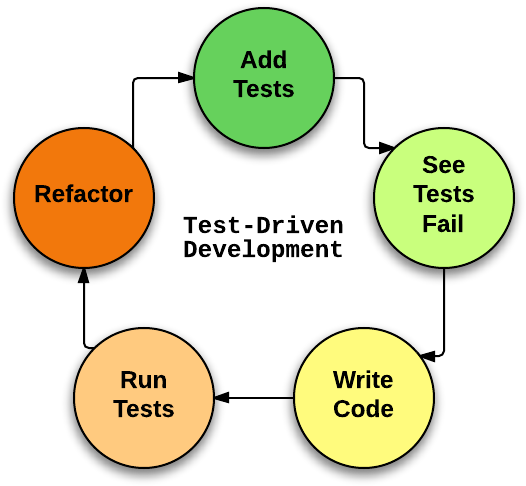
\includegraphics[scale=0.35]{images/TDD.png}
	\caption[Fluxograma Desenvolvimento Orientado a Testes(TDD)]{Fluxograma Desenvolvimento Orientado a Testes(TDD)\footnotemark}
\end{figure}
\footnotetext{Imagem obtida através de \url{https://www.clipartmax.com/middle/m2i8m2m2K9K9N4i8_bdd-flow-diagram-images-gallery-diagram/}}

\newpage
\paragraph{Processo Test Driven Development}
\begin{itemize}
	\item Escrever um teste que define uma nova função ou melhoria;
	\item Escrever a quantidade mínima de código para passar no teste;
	\item Refatorar o código para remover duplicações e melhorar seu design.
\end{itemize}

\paragraph{Benefícios Test Driven Development}
\begin{itemize}
	\item Tempo de trabalho reduzido: O TDD não permite que novo código seja escrito, a menos que o código existente seja testado com sucesso e sem falhas. Até que as falhas sejam completamente resolvidas e removidas, o processo de escrita do código é interrompido;
	\item Rápido feedback: Como os testes focam-se em secções especificas do código, os programadores podem receber feedback mais rapidamente permitindo-lhes implementar alterações de maneira mais eficiente;
	\item Maior produtividade de desenvolvimento: Com o TDD, o foco está na produção de código funcional, e não no design de casos de teste;
	\item Código mais flexível e de fácil manutenção: Como cada parte do código é testada antes de passar para a próxima parte do processo de desenvolvimento de software, o código mantém a funcionalidade e é adaptável no futuro.
\end{itemize}

\newpage
\subsubsection{Behavior-Driven Development}
O Desenvolvimento Orientado ao Comportamento (BDD) é uma extensão do TDD que reforça testar o comportamento da aplicação do ponto de vista do utilizador final. O BDD envolve a criação de especificações executáveis que definem o comportamento da aplicação. Este, baseia-se em testar comportamentos em vez de detalhes de implementação, facilitando a colaboração entre programadores, testers e utilizadores. Os cenários de BDD geralmente são descritos num formato mais legível e centrado ao utilizador, permitindo que utilizadores não programadores possam compreender os testes.

\paragraph{Processo Behavior-Driven Development}
As etapas para o Desenvolvimento Orientado ao Comportamento são bastante simples:

\begin{itemize}
	\item O comportamento é descrito normalmente utilizando uma user story, que permite que a equipa discuta exemplos concretos da nova funcionalidade e as expectativas do seu comportamento;
	\item A ação é então escrita, transformando os exemplos em documentação de forma que possa ser automatizada;
	\item O teste é executado para auxiliar e orientar os programadores no desenvolvimento do código;
	\item O código é então criado, para realizar esta funcionalidade tornando assim o código funcional.
\end{itemize}

\paragraph{Benefícios Behavior-Driven Development}
Existem vários benefícios em usar BDD para desenvolvimento de software, incluindo:

\begin{itemize}
	\item Incorporação da experiência do utilizador(UX): o BDD foca-se na experiência do utilizador, como tal, permite que a equipa desenvolva uma perspetiva mais ampla e observe lacunas no seu design;
	\item Custo-benefício: Como o BDD estabelece prioridades para utilizadores, programadores e investidores, este, permite que os recursos sejam utilizados de forma otimizada no desenvolvimento de software;
	\item Testes simples entre browsers: o BDD concentra-se no comportamento de utilizador, o que significa que oferece uma estrutura ideal para testes entre browsers.
\end{itemize}

\newpage
\subsubsection{TDD e BDD}
Em resumo, o TDD é uma prática de desenvolvimento que se foca em testar o código de forma isolada, enquanto o BDD é uma metodologia de equipa que se foca em testar o comportamento da aplicação do ponto de vista do utilizador. Embora partilhem semelhanças, eles têm algumas diferenças-chave na finalidade, no tipo de colaboração, na linguagem e nos casos de teste.

\vspace{1cm}
\begin{figure}[H]
	\centering
	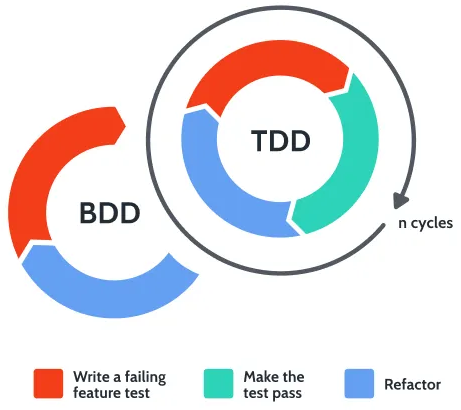
\includegraphics[scale=0.7]{images/tdd-bdd.png}
	\caption[Fluxograma TDD com BDD]{Fluxograma TDD com BDD\footnotemark}
\end{figure}
\footnotetext{Imagem obtida através de \url{https://www.outsystems.com/blog/posts/using-bdd-tdd/}}

\newpage
\subsection{Resultados}
Após efetuarmos os testes unitários ao código-fonte, corrermos o comando \verb"npx jest --coverage" e verificamos que conseguimos obter uma code coverage de cerca 95\%.

\scriptsize
\begin{verbatim}
-----------------------------|---------|----------|---------|---------|-------------------------------------
File                         | % Stmts | % Branch | % Funcs | % Lines | Uncovered Line #s
-----------------------------|---------|----------|---------|---------|-------------------------------------
All files                    |   91.34 |     78.2 |   95.12 |   91.34 |
 scripts                     |   86.88 |    76.78 |   90.24 |   86.88 |
  authentication-handlers.js |     100 |      100 |     100 |     100 |
  clients-handlers.js        |     100 |      100 |     100 |     100 |
  globalHandlers.js          |     100 |      100 |     100 |     100 |
  jobs-handlers.js           |   85.84 |    67.85 |     100 |   85.84 | 40-48,94-96,101,121-126,154-156,165
  messaging-handlers.js      |   74.28 |    66.66 |   66.66 |   74.28 | 57-78
  users-handlers.js          |   82.97 |       80 |      80 |   82.97 | 77-86
 tests                       |   95.85 |       79 |     100 |   95.85 |
  classes-code.js            |     100 |      100 |     100 |     100 |
  localStorage-code.js       |   89.47 |    76.47 |     100 |   89.47 | 29,43,58,72,87,101,116,130
  requests-code.js           |    98.4 |     80.3 |     100 |    98.4 | 94-95
-----------------------------|---------|----------|---------|---------|-------------------------------------
\end{verbatim}
\normalsize

Podemos observar que relativamente ao ficheiro \verb"localStorage-code.js" as linhas não cobertas estão relacionadas com verificações à propriedade \textit{localStorage}, que no ambiente de testes esteve \textit{"mocked"}, por forma a não mexer com dados originais. Ainda no ficheiro \verb"request-code.js", as linhas não cobertas estão relacionadas com o insucesso do pedido de \textit{logout} pois num ambiente de produção o servidor retornava sempre o resultado \textit{status: 200}.

Desta forma, deixamos nos anexos o report do resultado individual de cada teste unitário.

\subsubsection{Testes sem Sucesso}
De seguida podemos analisar os testes que falharam, de uma forma breve iremos explicar o porquê.
\begin{itemize}
	\item Delete User tests(handle an unsuccessful user delete because of missing data) - Este teste falhou pois não é efetuado a validação do parâmetro ID;
	\item getUsersAjax function tests (With unsuccessful request and new users saved in localStorage) - Este teste falhou devido ao mau tratamento de dados. Quando o servidor consegue ler os dados da base de dados, este envia um objeto JSON para o cliente e este é devolvido. Quando o servidor não consegue ler os dados da base de dados, a request vai buscar os dados guardados no localStorage, mas o localStorage guarda os dados em String e a função de request devolve os dados sem fazer o parse para objeto;
	\item getClientsAjax function tests (With unsuccessful request and new users saved in localStorage) - Este teste falhou devido ao mau tratamento de dados. Quando o servidor consegue ler os dados da base de dados, este envia um objeto JSON para o cliente e este é devolvido. Quando o servidor não consegue ler os dados da base de dados, a request vai buscar os dados guardados no localStorage, mas o localStorage guarda os dados em String e a função de request devolve os dados sem fazer o parse para objeto.
\end{itemize}

\newpage
\section{Anexos}
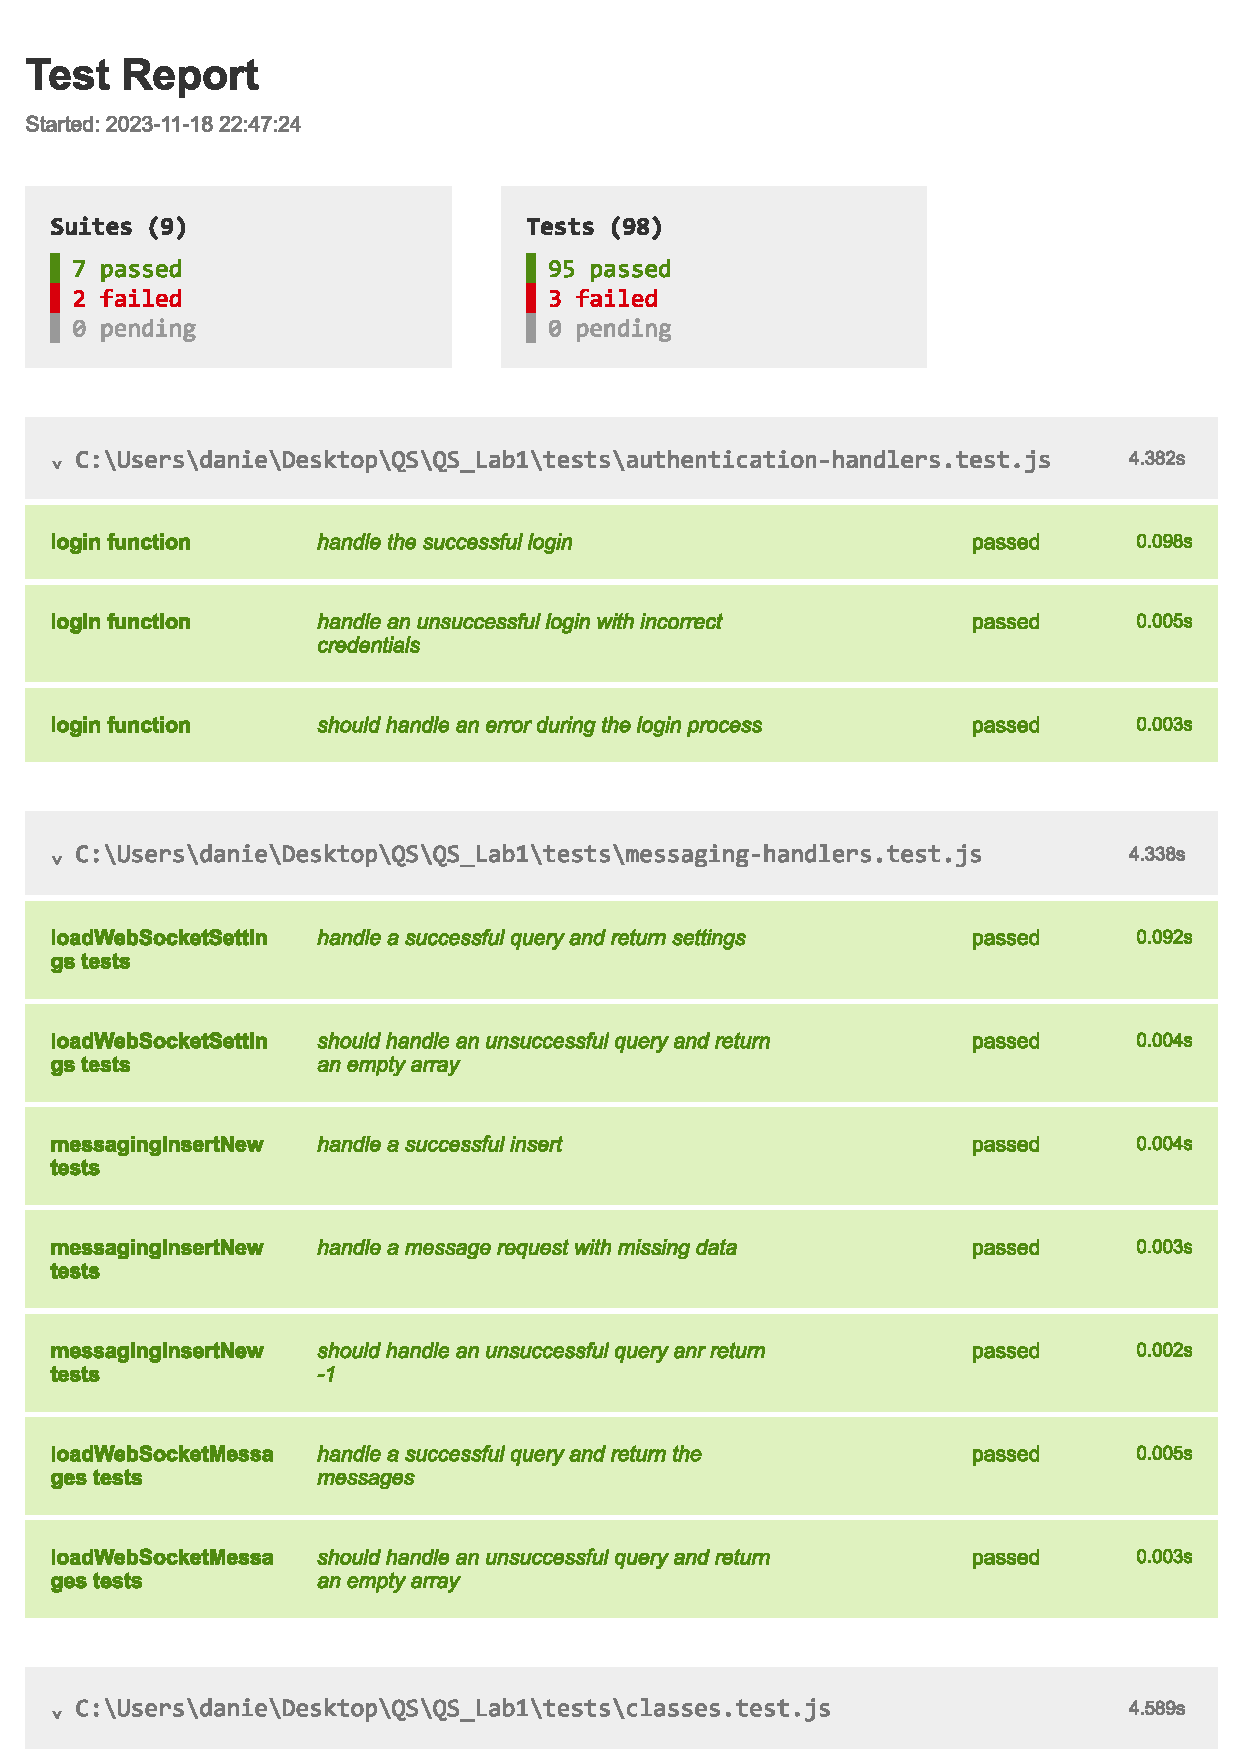
\includepdf[pages=-]{../reports/test_report.pdf}

\end{document}
